\documentclass[tikz, border=1cm]{standalone}
\usepackage{pgfplots}
\pgfplotsset{compat=1.18}
\usepgfplotslibrary{patchplots}
\begin{document}

  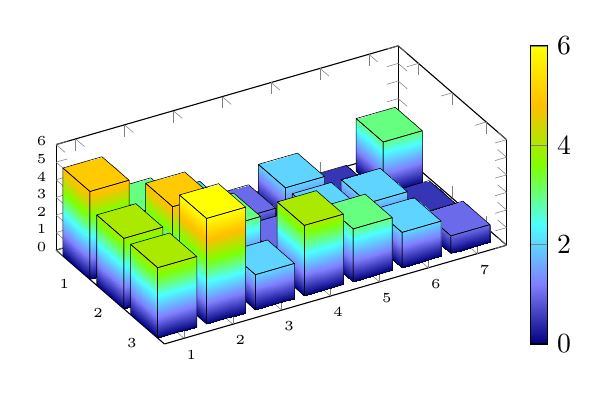
\begin{tikzpicture}
    \newcommand{\barw}{0.4}
    \newcommand{\boxbar}[3]{
    \addplot3[
      patch, 
      shader=interp,
      patch type=rectangle,
      patch refines=2,
    ]
    coordinates { (#1-\barw,#2-\barw,0) (#1-\barw,#2-\barw,#3) (#1+\barw,#2-\barw,#3) (#1+\barw,#2-\barw,0) (#1-\barw,#2-\barw,#3) (#1-\barw,#2+\barw,#3) (#1+\barw,#2+\barw,#3) (#1+\barw,#2-\barw,#3) (#1+\barw,#2-\barw,0) (#1+\barw,#2-\barw,#3) (#1+\barw,#2+\barw,#3) (#1+\barw,#2+\barw,0)};  
    \addplot3[
      patch, 
      patch type=rectangle,
      mesh, black, very thin,
    ]
    coordinates { (#1-\barw,#2-\barw,0) (#1-\barw,#2-\barw,#3) (#1+\barw,#2-\barw,#3) (#1+\barw,#2-\barw,0) (#1-\barw,#2-\barw,#3) (#1-\barw,#2+\barw,#3) (#1+\barw,#2+\barw,#3) (#1+\barw,#2-\barw,#3) (#1+\barw,#2-\barw,0) (#1+\barw,#2-\barw,#3) (#1+\barw,#2+\barw,#3) (#1+\barw,#2+\barw,0)};
    }

    \begin{axis}[
      colormap={CM}{
        color=(blue!50!black)
        color=(blue!50!white)
        color=(cyan!70!white)
        color=(green!50!yellow)
        color=(orange!50!yellow)
        color=(yellow)
      },
      view={60}{30},
      unit vector ratio=1.2 1 0.6,
      xmin=0.4, xmax=3.6,
      ymin=0.6, ymax=7.6,
      zmin=0, zmax=6,
      colorbar, colorbar/width=6pt,
      xtick distance=1, ytick distance=1, ztick distance=1,
      font=\tiny,
    ]

      \foreach \myz [count=\i] in {3,0.5,2,1,2,3,5} {
      \boxbar{1}{8-\i}{\myz}}

      \foreach \myz [count=\i] in {0.5,2,2,1,3,5,4}{
      \boxbar{2}{8-\i}{\myz}}

      \foreach \myz [count=\i] in {1,2,3,4,2,6,4}{
      \boxbar{3}{8-\i}{\myz}}

    \end{axis}
  \end{tikzpicture}
\end{document}
